
\section{OpenLearning}
\subsection{Overview}
OpenLearning is a ASX listed company that provides an LMS for educational providers. It was founded by Adam Brino, Richard Buckland (COMP6441 lecturer) and David Collien and is used in security courses at UNSW.\\
It works with universities such as UNSW and Taylor's University (based in Malaysia) to deliver MOOCs (massive open online courses). It also features an LMS that educational institutions can use. Some courses at UNSW currently use it such as COMP6441 (Security), and many universities such as UNSW, UTS, ACU, Charles Sturt University and more also use the platform.\\
Unlike other content management systems such as Moodle, OpenLearning is not free or open source and can be quite costly.\\

\subsection{Home}
When logged in, the home page of OpenLearning is quite confusing.\\
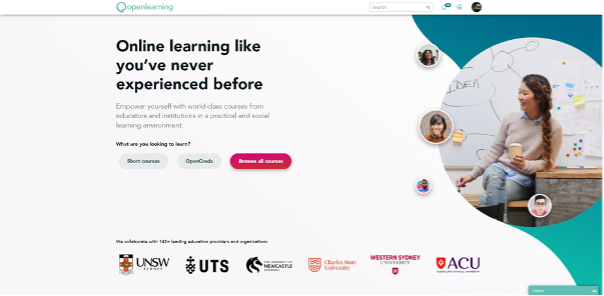
\includegraphics{openlearning-homepage} \\
For students, it can be quite confusing how to reach their courses. The home page clearly directs you to search for a new course offered by OpenLearning, not a course you are already enrolled in. \\

